\section{Hardware Optimisations}
\label{sec:hardware optimisations}

\subsection{Testing Warp Sizes}
\label{sec:testing warp sizes}

In \cref{sec:gpu} we introduced the concept of a warp, a scheduler for launching threads within a kernel.
\cref{tab:warp size testing} shows the average elapsed time over 1,000 runs for launching different threads, to see the impact compared to the amount of warps are needed.
One warp launches 32 threads at a time, asserted from \cref{ap:tesla k40 specifications}.

\begin{table}[htb]%
  \begin{minipage}{0.49\linewidth}
    \centering
    \begin{tabular}{lrr}
      \toprule
      threads (\#) & time (ms) & latency \\
      \midrule
      $32 \times 10$    & $5.321$ &          \\
      $32 \times 10-1$  & $5.336$ & $+0.28\%$  \\
      $32 \times 10-16$ & $5.600$ & $+5.24\%$  \\
      $32 \times 10-31$ & $5.892$ & $+10.73\%$ \\
      \bottomrule
    \end{tabular}
  \end{minipage}%
  \begin{minipage}{0.49\linewidth}
    \centering
    \begin{tabular}{lrr}
      \toprule
      threads (\#) & time (ms) & latency \\
      \midrule
      $32 \times 9$     & $5.561$ & \\
      $32 \times 9-1$   & $5.585$ & $+0.43\%$  \\
      $32 \times 9-16$  & $5.892$ & $+5.95\%$  \\
      $32 \times 9-31$  & $6.236$ & $+12.13\%$ \\
      \bottomrule
    \end{tabular}
  \end{minipage}%
  \caption{Testing different warp sizes}
  \label{tab:warp size testing}
\end{table}

We present the multiple of 32 as the base case for the two tables.
By using block size between $32 \times 8$ and $32 \times 9$ the SM still launched the same amount of warps (9 warps per block), but with idle threads in the 9'th warp as it must have 32 threads.
As the amount of threads per block is reduced the total amount of blocks nessesary to complete the job must increase and thus increases runtime.
\cref{tab:warp size testing} shows how the performance deteriorates as the amount of idle threads in the last warp increases.

\subsection{Testing BUS width}
\label{sec:testing BUS width}

In \cref{sec:gpu} we introduced the concept of a warp, a scheduler for launching threads within a kernel.
\cref{fig:block size testing} shows the average elapsed time over 10 runs for launching different block size being multiples of the warp size, to see the SM's max thread bottleneck is impacted the impact by the amount of threads in a block.
The SM can handle 2048 threads concurrently, asserted from \cref{ap:tesla k40 specifications}.
Active threads in \cref{fig:active threads}.
\todo{flat 2048 curve}

\begin{figure*}[t]
  \centering
  \begin{subfigure}[b]{.49\linewidth}
    \centering
    \resizebox{!}{.80\textwidth}{
      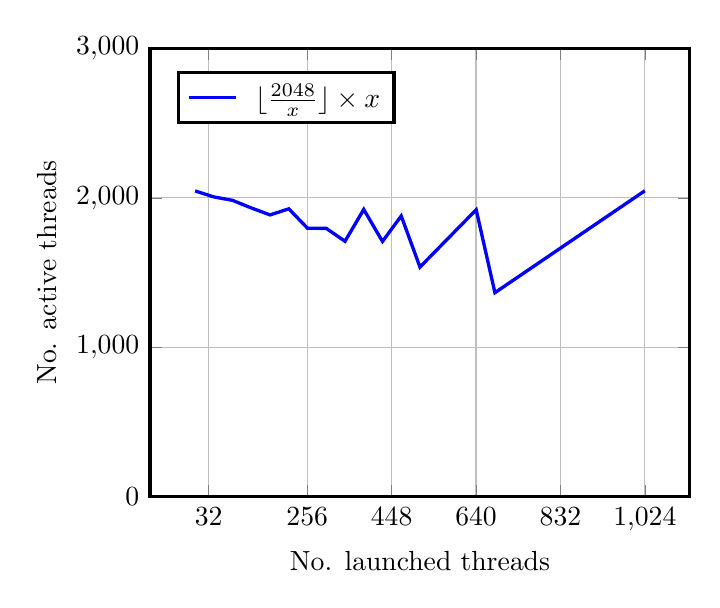
\begin{tikzpicture}
  \begin{axis}[
    ymajorgrids,
    xmajorgrids,
    ymin=0,ymax=3000,
    xtick={32,256,448,640,832,1024},
    ylabel={No. active threads},
    xlabel={No. launched threads},
%    xmode=log,
%    log basis x={2},
    legend style={
      at={(0.05,0.95)},
      anchor=north west,
      column sep=1ex
     },
     no markers,
     very thick 
   ]

   \addplot+[domain=1:1024] {floor((2048/x))*x};
   \addlegendentry{$\lfloor \frac{2048}{x} \rfloor \times x $};
  \end{axis}
\end{tikzpicture}

    }
    \caption{Active threads vs. launched threads}
    \label{fig:active threads}
  \end{subfigure}%
  ~
  \begin{subfigure}[b]{.49\linewidth}
    \centering
    \resizebox{!}{.80\textwidth}{
      \begin{tikzpicture}
  \begin{axis}[
    ymajorgrids,
    xmajorgrids,
    ymax=35,
    xtick={32,256,448,640,832,1024},
    ylabel={Time (ms)},
    xlabel={No. threads},
    legend style={
      at={(0.05,0.95)},
      anchor=north west,
      column sep=1ex
     },
     no markers,
     very thick 
   ]

    \addplot table [x=threads, y=time] {data/threadsperblock.csv};
    \addlegendentry{mapping $2^{29}$ values};
  \end{axis}
\end{tikzpicture}

    }
    \caption{Mapping $2^{29}$ values}
    \label{fig:block size testing}
  \end{subfigure}%
  \caption{Threads and warps}
  \label{fig:threads and warps}
\end{figure*}

%\begin{table}[htb]%
%  \begin{minipage}{0.49\linewidth}
%    \centering
%    \begin{tabular}{lrr}
%      \toprule
%      threads (\#) & time (ms) & latency \\
%      \midrule
%      $32 \times 10$    & $5.321$ &          \\
%      $32 \times 10-1$  & $5.336$ & $+0.28\%$  \\
%      $32 \times 10-16$ & $5.600$ & $+5.24\%$  \\
%      $32 \times 10-31$ & $5.892$ & $+10.73\%$ \\
%      \bottomrule
%    \end{tabular}
%  \end{minipage}%
%  \begin{minipage}{0.49\linewidth}
%    \centering
%    \begin{tabular}{lrr}
%      \toprule
%      threads (\#) & time (ms) & latency \\
%      \midrule
%      $32 \times 9$     & $5.561$ & \\
%      $32 \times 9-1$   & $5.585$ & $+0.43\%$  \\
%      $32 \times 9-16$  & $5.892$ & $+5.95\%$  \\
%      $32 \times 9-31$  & $6.236$ & $+12.13\%$ \\
%      \bottomrule
%    \end{tabular}
%  \end{minipage}%
%  \caption{Testing different warp sizes}
%  \label{tab:warp size testing}
%\end{table}

As visable in the graph it has a "wave" function.
Further is a function of the total amount of threads the SM can execute on.
There is a clear correlation, which indicates that choosing a block size that maximizes the amount of threads able to concurrently execute is essential to achieving the best performance.
